\documentclass[../thesis.tex]{subfiles}
\begin{document}

\chapter{Results}
\label{ch:results}

This section summarizes the results of the analysis, starting with the pairwise Mood's Median tests followed by the results of the modeling process. Results are compared with the work of Horne et al. and Gruppi et al. to highlight overlaps and disagreements between their results and the results of this paper.

\section{Mood's Median Test}

For each feature described in \ref{methodology}, a Mood's Median Test was used to test for differences between real and fake news. The table below includes the result of these tests, excluding tests with resulting p-values of $>0.05$. For each predictor, the p-value of the test is given, along with a comparison of the groupwise medians to indicate which group is higher. Furthermore, as many of the features used in this paper are also used in O'Brien et al. and Gruppi et al., we indicate, when available, whether the results of these tests agree with the results found in both papers. As both papers First, a table including results for the body of articles is included, then for the titles. 

\begin{longtable}[t]{lllll}
\caption{\label{tab:}Mood's Median Test Results for Article Body}\\
\toprule
Variable & Result & p-value & Gruppi et al. & Obrien et al.\\
\midrule
mu\_sentence & Real > Fake & < 0.001 & - & Disagree\\
mu\_verb\_phrase & Real > Fake & < 0.001 & - & -\\
num\_verb\_phrase & Fake > Real & < 0.05 & - & -\\
swc & Real > Fake & < 0.001 & - & -\\
types & Fake > Real & < 0.05 & - & -\\
\addlinespace
tokens & Fake > Real & < 0.001 & - & -\\
TTR & Real > Fake & < 0.001 & - & Disagree\\
FOG & Real > Fake & < 0.001 & - & -\\
SMOG & Real > Fake & < 0.001 & Agree & -\\
FK & Real > Fake & < 0.001 & Disagree & Agree\\
\addlinespace
CL & Fake > Real & < 0.01 & - & -\\
ARI & Real > Fake & < 0.001 & - & -\\
WC & Fake > Real & < 0.01 & Disagree & -\\
Tone & Fake > Real & < 0.001 & - & -\\
WPS & Real > Fake & < 0.001 & Agree & -\\
\addlinespace
shehe & Real > Fake & < 0.001 & Agree & Disagree\\
article & Real > Fake & < 0.001 & - & -\\
prep & Real > Fake & < 0.001 & - & -\\
auxverb & Real > Fake & < 0.05 & Agree & -\\
conj & Fake > Real & < 0.001 & - & -\\
\addlinespace
posemo & Fake > Real & < 0.001 & - & -\\
negemo & Real > Fake & < 0.001 & - & -\\
anger & Real > Fake & < 0.001 & - & -\\
male & Real > Fake & < 0.001 & - & -\\
cogproc & Fake > Real & < 0.001 & - & -\\
\addlinespace
insight & Real > Fake & < 0.05 & - & -\\
discrep & Fake > Real & < 0.05 & - & -\\
differ & Fake > Real & < 0.01 & - & -\\
percept & Real > Fake & < 0.05 & - & -\\
see & Real > Fake & < 0.001 & - & -\\
\addlinespace
hear & Real > Fake & < 0.001 & - & -\\
feel & Real > Fake & < 0.01 & - & -\\
bio & Real > Fake & < 0.001 & - & -\\
body & Real > Fake & < 0.01 & - & -\\
health & Real > Fake & < 0.05 & - & -\\
\addlinespace
drives & Fake > Real & < 0.001 & - & -\\
affiliation & Fake > Real & < 0.001 & - & -\\
achieve & Fake > Real & < 0.001 & - & -\\
focuspast & Real > Fake & < 0.001 & - & -\\
focuspresent & Fake > Real & < 0.001 & - & -\\
\addlinespace
relativ & Real > Fake & < 0.01 & - & -\\
time & Real > Fake & < 0.001 & - & -\\
work & Fake > Real & < 0.05 & - & -\\
leisure & Real > Fake & < 0.001 & - & -\\
money & Fake > Real & < 0.001 & - & -\\
\addlinespace
AllPunc & Fake > Real & < 0.01 & - & -\\
Period & Fake > Real & < 0.001 & - & -\\
Dash & Fake > Real & < 0.01 & - & -\\
Quote & Real > Fake & < 0.001 & - & Agree\\
Apostro & Real > Fake & < 0.05 & - & -\\
\addlinespace
Parenth & Fake > Real & < 0.01 & - & -\\
CC & Fake > Real & < 0.01 & - & -\\
DT & Fake > Real & < 0.05 & - & Disagree\\
IN & Fake > Real & < 0.05 & - & -\\
JJ & Fake > Real & < 0.01 & - & -\\
\addlinespace
MD & Fake > Real & < 0.05 & - & -\\
NN & Fake > Real & < 0.001 & - & Disagree\\
NNS & Fake > Real & < 0.001 & - & -\\
NNP & Fake > Real & < 0.05 & - & -\\
NNPS & Fake > Real & < 0.001 & - & -\\
\addlinespace
TO & Fake > Real & < 0.001 & - & -\\
VB & Fake > Real & < 0.05 & - & -\\
VBN & Fake > Real & < 0.01 & - & -\\
VBP & Fake > Real & < 0.05 & - & -\\
VBZ & Fake > Real & < 0.01 & - & -\\
\addlinespace
NER & Real > Fake & < 0.001 & - & -\\
len & Fake > Real & < 0.001 & - & -\\
\bottomrule
\end{longtable}

Despite significant overlap in features used with two comparable papers, particularly O'Brien et al., very few features significant in this paper's tests were also significant in the other two studies. Furthermore, when features were significant in both cases, they frequently disagreed, in many cases even demonstrating agreement for one study and disagreement in another. The only clear agreements were the SMOG complexity score, mean words per sentence, auxiliary verbs per 100 words, and quotes per 100 words with respect to the body of articles.

Next, the results for the same tests and features with respect to the title of articles is shown below. As Gruppi et al. do not model at the title level, only comparisons with O'Brien et al. are included.

\begin{longtable}[t]{llll}
\caption{\label{tab:}Mood's Median Test Results for Article Title}\\
\toprule
Variable & Result & p-value & Obrien et al.\\
\midrule
mu\_sentence & Real > Fake & < 0.001 & -\\
mu\_verb\_phrase & Real > Fake & < 0.001 & -\\
mu\_noun\_phrase & Real > Fake & < 0.05 & -\\
sd\_noun\_phrase & Real > Fake & < 0.05 & -\\
num\_verb\_phrase & Real > Fake & < 0.001 & -\\
\addlinespace
types & Real > Fake & < 0.001 & -\\
tokens & Real > Fake & < 0.001 & -\\
TTR & Fake > Real & < 0.001 & -\\
SMOG & Real > Fake & < 0.001 & -\\
FK & Real > Fake & < 0.05 & Agree\\
\addlinespace
CL & Fake > Real & < 0.01 & -\\
ARI & Real > Fake & < 0.05 & -\\
WC & Real > Fake & < 0.001 & -\\
WPS & Real > Fake & < 0.001 & Disagree\\
function. & Real > Fake & < 0.001 & -\\
\addlinespace
prep & Real > Fake & < 0.05 & -\\
verb & Real > Fake & < 0.001 & -\\
social & Real > Fake & < 0.001 & -\\
space & Real > Fake & < 0.05 & -\\
NNP & Real > Fake & < 0.001 & Disagree\\
\addlinespace
len & Real > Fake & < 0.001 & -\\
\bottomrule
\end{longtable}

Similarly to the tests describing the body of articles, there was little overlap between significant results in this paper and in the work of O'Brien et al, with only three features significant in both. Additionally, the pattern of disagreement continued, with two out of the three overlapping results in disagreement. The only result shared between this paper and O'Brien et al. was that the FK complexity score is higher in real articles than fake articles.

\section{Modeling}

While the results of the Mood's Median Tests demonstrate where real and fake articles differ, on median, at the level of each feature, it does not provide a meaningful way to predict the class of an article based on these textual features. While we expect features with significant tests to be quality predictors, this is not always the case. This section thus highlights the most important and impactful predictors of fake news, utilizing the coefficients and AUC-based variable importance. The overall predictive accuracy of each model is also described and compared to prior work with the FNN dataset, to demonstrate the efficacy of this paper's model.

The final body-level model included X features after the Lasso regression shrunk Y features to 0. This model performs quite well, with an AUC of 0.85, and a accuracy of 76\% relative to a 50\% baseline, as well as sensitivity and specificity of 0.74 and 0.78 with a cutoff of 0.5. This is close to - INSERT REFERENCE TO COMPARABLE RESULTS

The most impactful and important features for the body-level model are shown in the following plot, with the coefficient magnitude shown on the x-axis and the AUC-based variable importance on the y-axis. Note that the baseline importance for a variable with no predictive power is 0.5, hence why the y-axis does not start at 0. Features with large variable importance scores have the most individual predictive power, while features with large coefficients having the largest effect on individual observations when these features take on values significantly away from the mean. Negative coefficients represent features indicative of real news, while positive ones are indicative of fake news. Note that only features with p-values of >0.1 are shown.

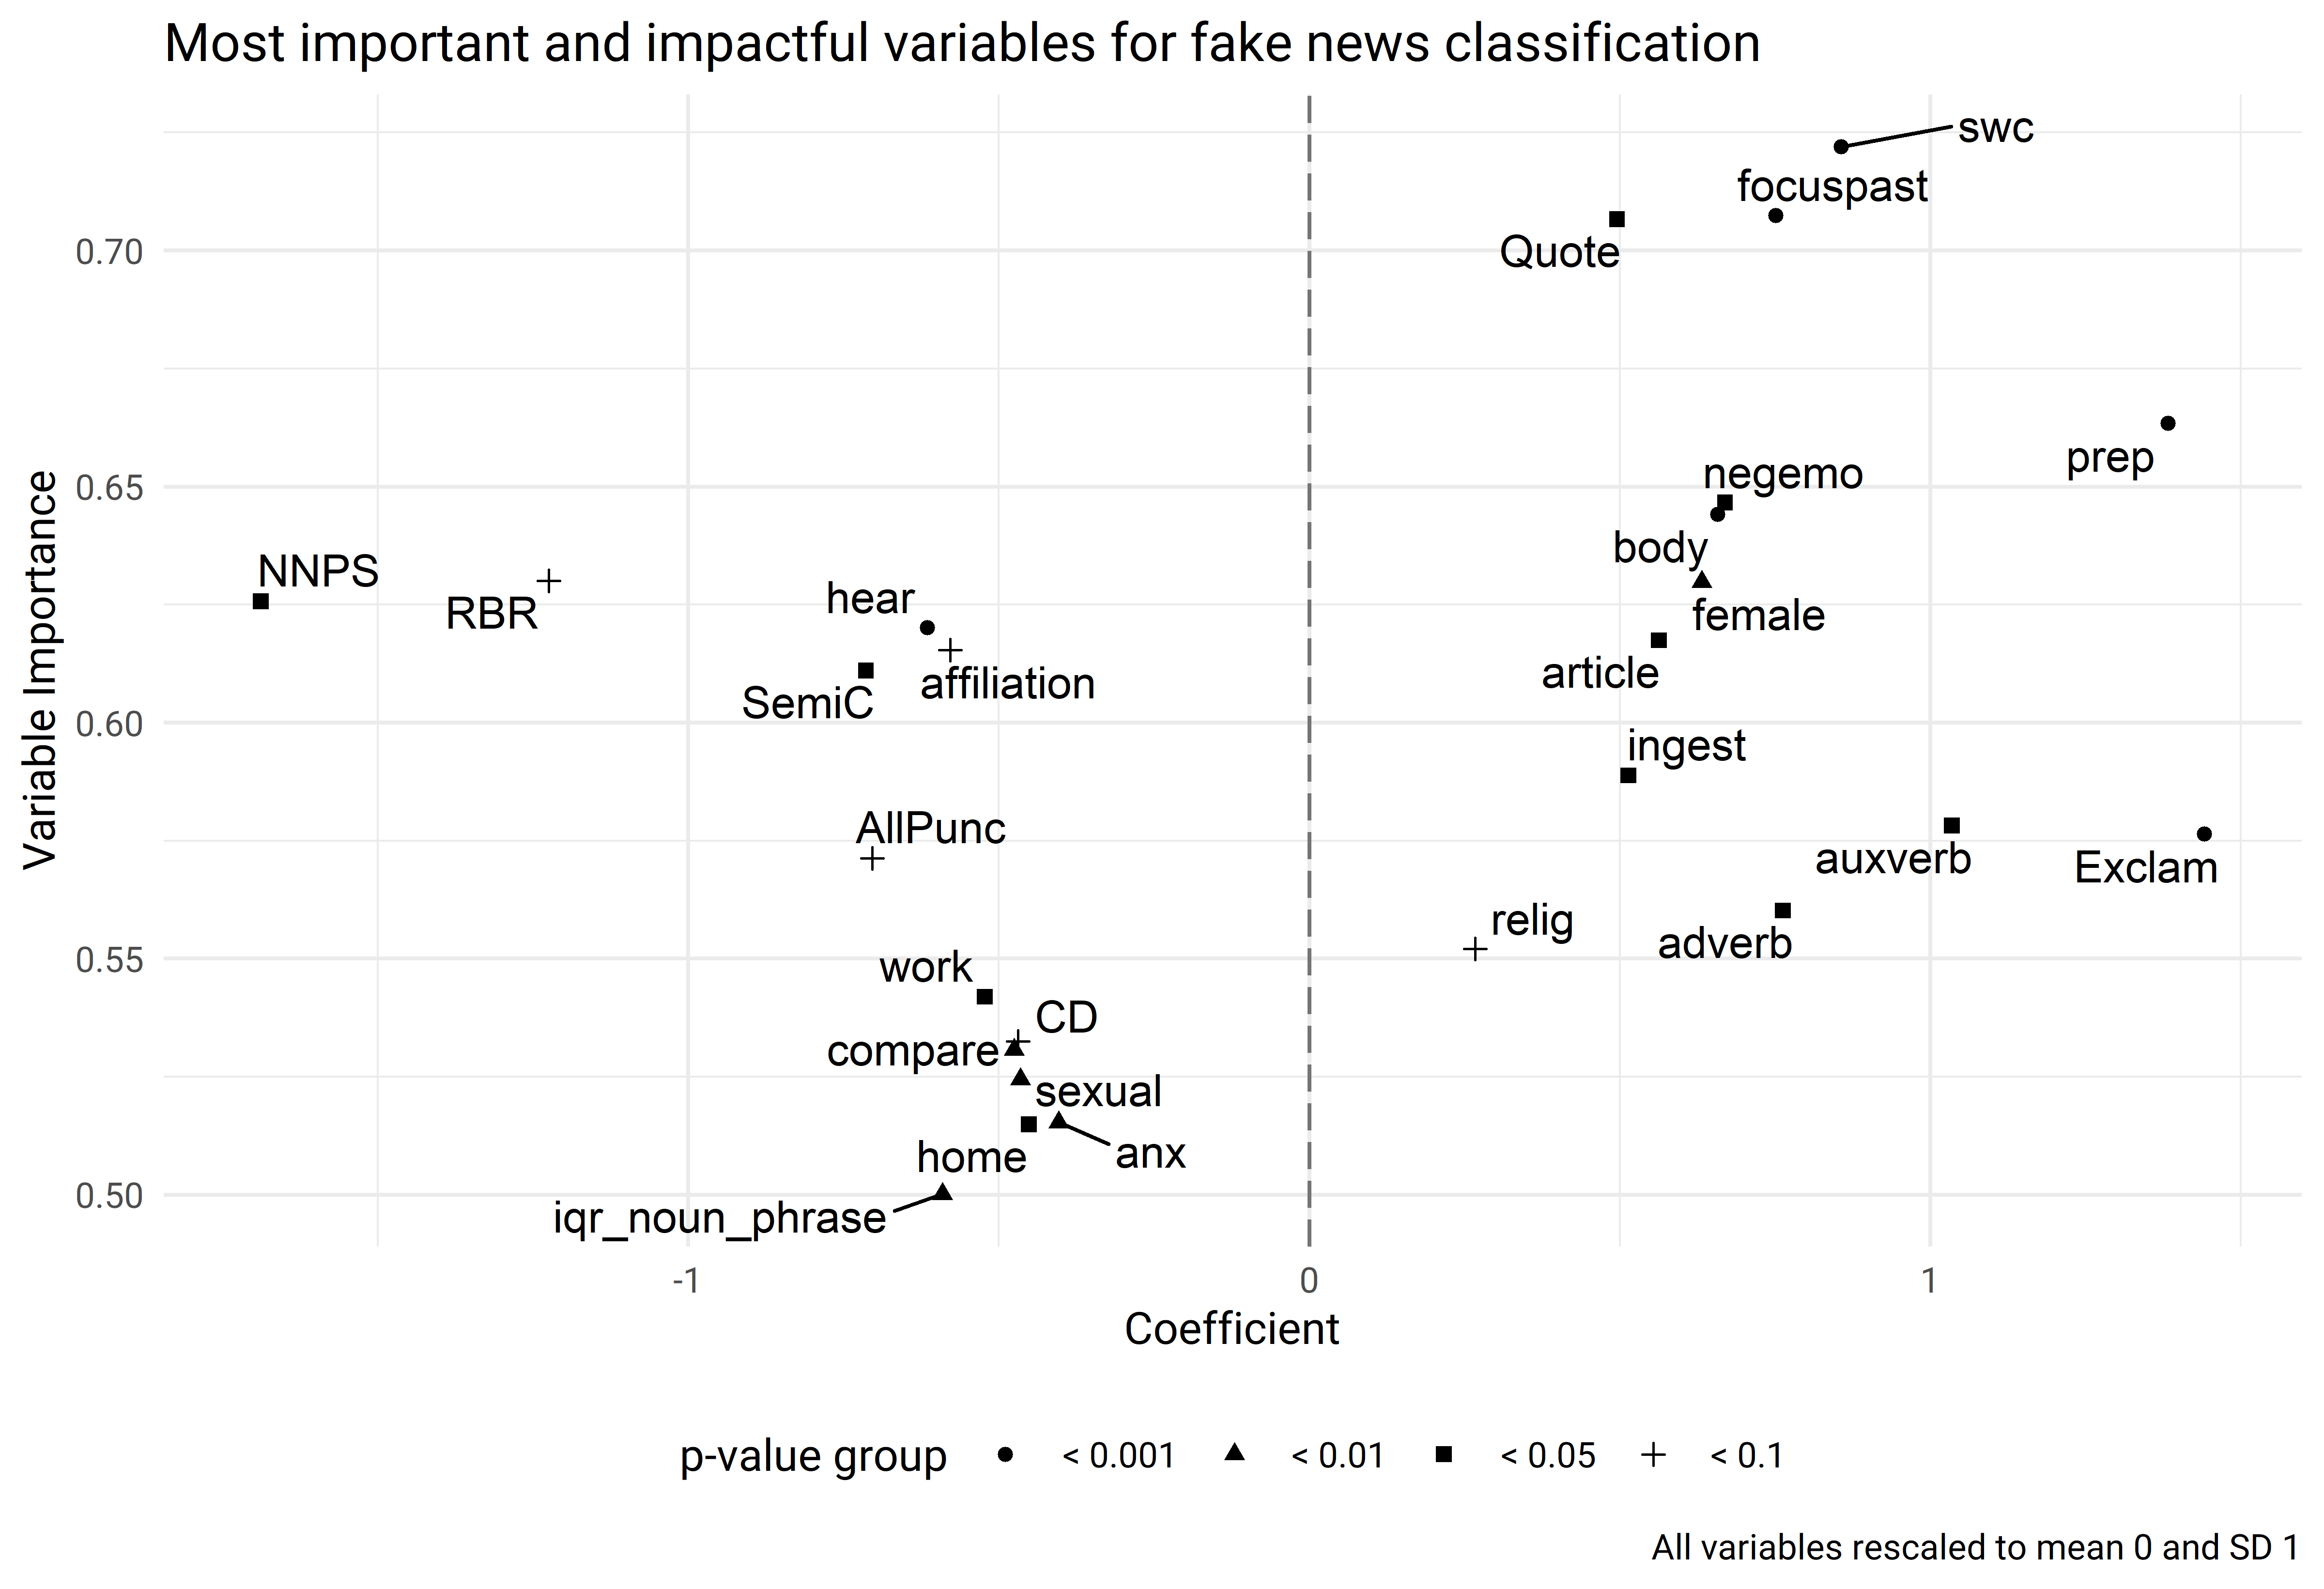
\includegraphics[scale=0.75]{body.png}

The above plot demonstrates that the most impactful predictors of fake news at the body-level are the usage of prepositions, auxiliary verbs, and exclamations.    Predictors indicating news is real are less numerous, with the most impactful being the usage of plural proper nouns. As for most important features, the usage of quotes and words focusing on the past above the mean are good individual predictors of fake news across the entire dataset, as well as the length of sentences.

The final title-level included X features after the Lasso regression shrunk Y features to 0. This model performs similarly to the body-level model, with an AUC of 0.835, and an accuracy of 77\% relative to a baseline of 50\%, as well as a sensitivity and specificity of 0.823 and 0.729 respectively, using a cutoff of 0.36 selecting using ROC curve analysis. Again, this accuracy is similar to prior work, comparable with the work of - INSERT COMPARABLE RESULTS

The same feature importance and impact plot created for the title-level model, and is shown below. The interpretation for this plot is the same as before. As before, only features  with p-values below 0.1 are shown.

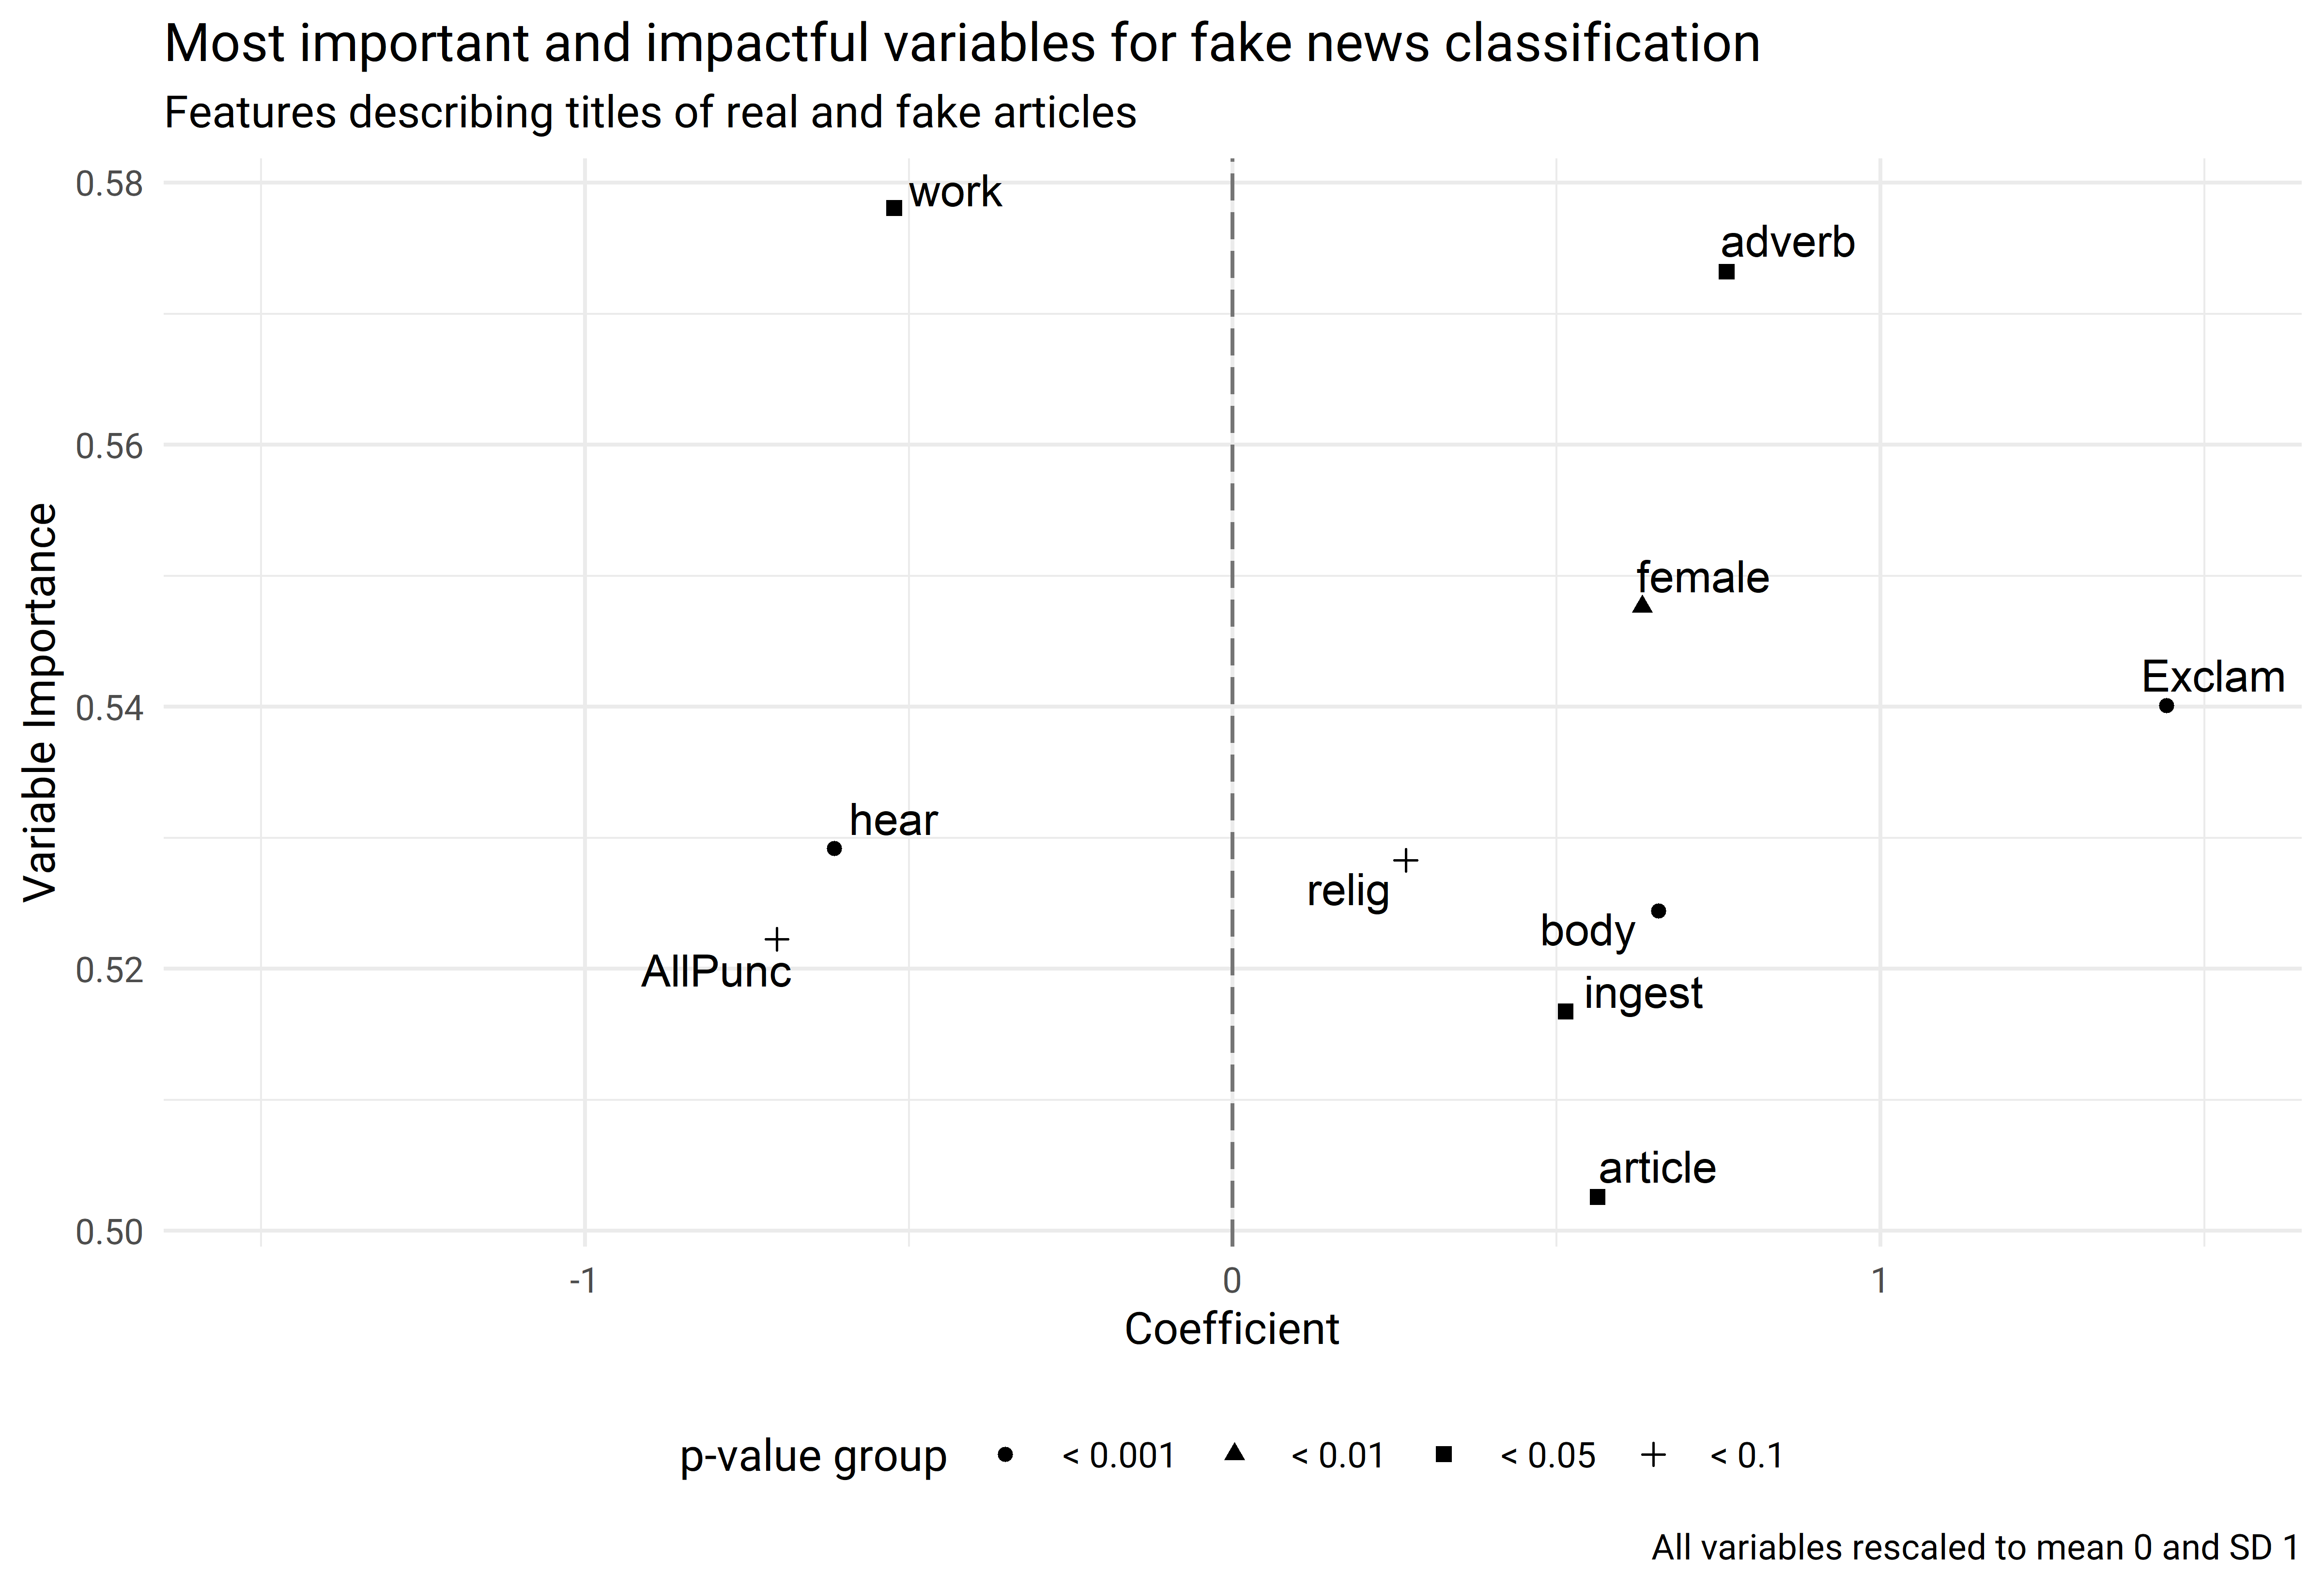
\includegraphics[scale=0.75]{titles.png}

Similarly to the results of the Mood's Median Tests, there are fewer significant features at the title-level than at the body-level. The most impactful predictor of fake news is again the usage of exclamation marks, suggesting it is a consistent point of difference between real and fake news. The most impactful predictors of real news are words relating to work, the perceptual process of hearing, and the usage of punctuation in general, though the latter is only marginally significant. The most important individual predictors are words relating to work, suggesting an article is real, and the usage of adverbs, suggesting an article is fake.

\end{document}
